
\section{Silicon Photomultipliers}
\label{sec.sipm}

When a photon travels through silicon (a semiconductor), it can transfer its energy to a bound state (valence) electron, pushing it into the conduction band and thus creating an electron-hole pair. Silicon is a good photo detector material in the spectral range form 350 nm up to 800 nm, e.g, at frequencies ranging from the deep blue to the red. 

In a silicon photodiode one applies a reverse bias to a p-n junction. A reverse bias is simply a voltage that counteracts the diffusive force that draws negative and positive charge carriers (electrons and holes respectively) to the depletion region situated around the p-n junction. Under application of the reverse bias, the diode is ``open'' (no flow of net charge) until it absorbs a photon. When this happens, electrons acquire enough energy to be pushed to the conduction band and as a  result a net current (electrons through the n-type and holes through the p-type sides of the device) appears in the diode.

When a sufficiently high electric field (> $5 \times 10^5$~ V/cm) is generated within the depletion region of the silicon, a charge carrier created in this region will be accelerated to a point where it carries sufficient kinetic energy to create secondary charge pairs through a process called impact ionization. In this way, a single photoelectron can trigger a self-perpetuating ionization cascade that will spread throughout the silicon volume subjected to the field. The silicon will break down and become conductive, effectively amplifying the original photoelectron into a macroscopic current flow. This process is called Geiger discharge, in analogy to the ionization discharge observed in a Geiger-Muller tube. 

A photodiode operated in Geiger mode employs this mechanism of breakdown to achieve a high gain. The p-n junction region is designed in such a way that it can sustain a reverse bias beyond its nominal breakdown voltage, creating the necessary high field gradients across the junction. Once a current is flowing it should then be stopped or ‘quenched’. Using passive quenching (i.e. no active circuitry), this is achieved through the means of a series resistor RQ which limits the current drawn by the diode during break down, and hence lowers the reverse voltage seen by the diode to a value below its breakdown voltage. Thus a cycle of breakdown, avalanche, quench and subsequent reset of the bias to a value above the breakdown voltage is achieved. In this way, a single photodiode device operated in Geiger-mode functions as a photon-triggered switch, in either an ``on'' or ``off'' state, and therefore cannot provide proportional information regarding the magnitude of an instantaneous photon flux. Regardless of the number of photons interacting within a diode at the same time, it will produce a signal of ``1'' photon.


\begin{figure}[!bhtp]
	\centering
	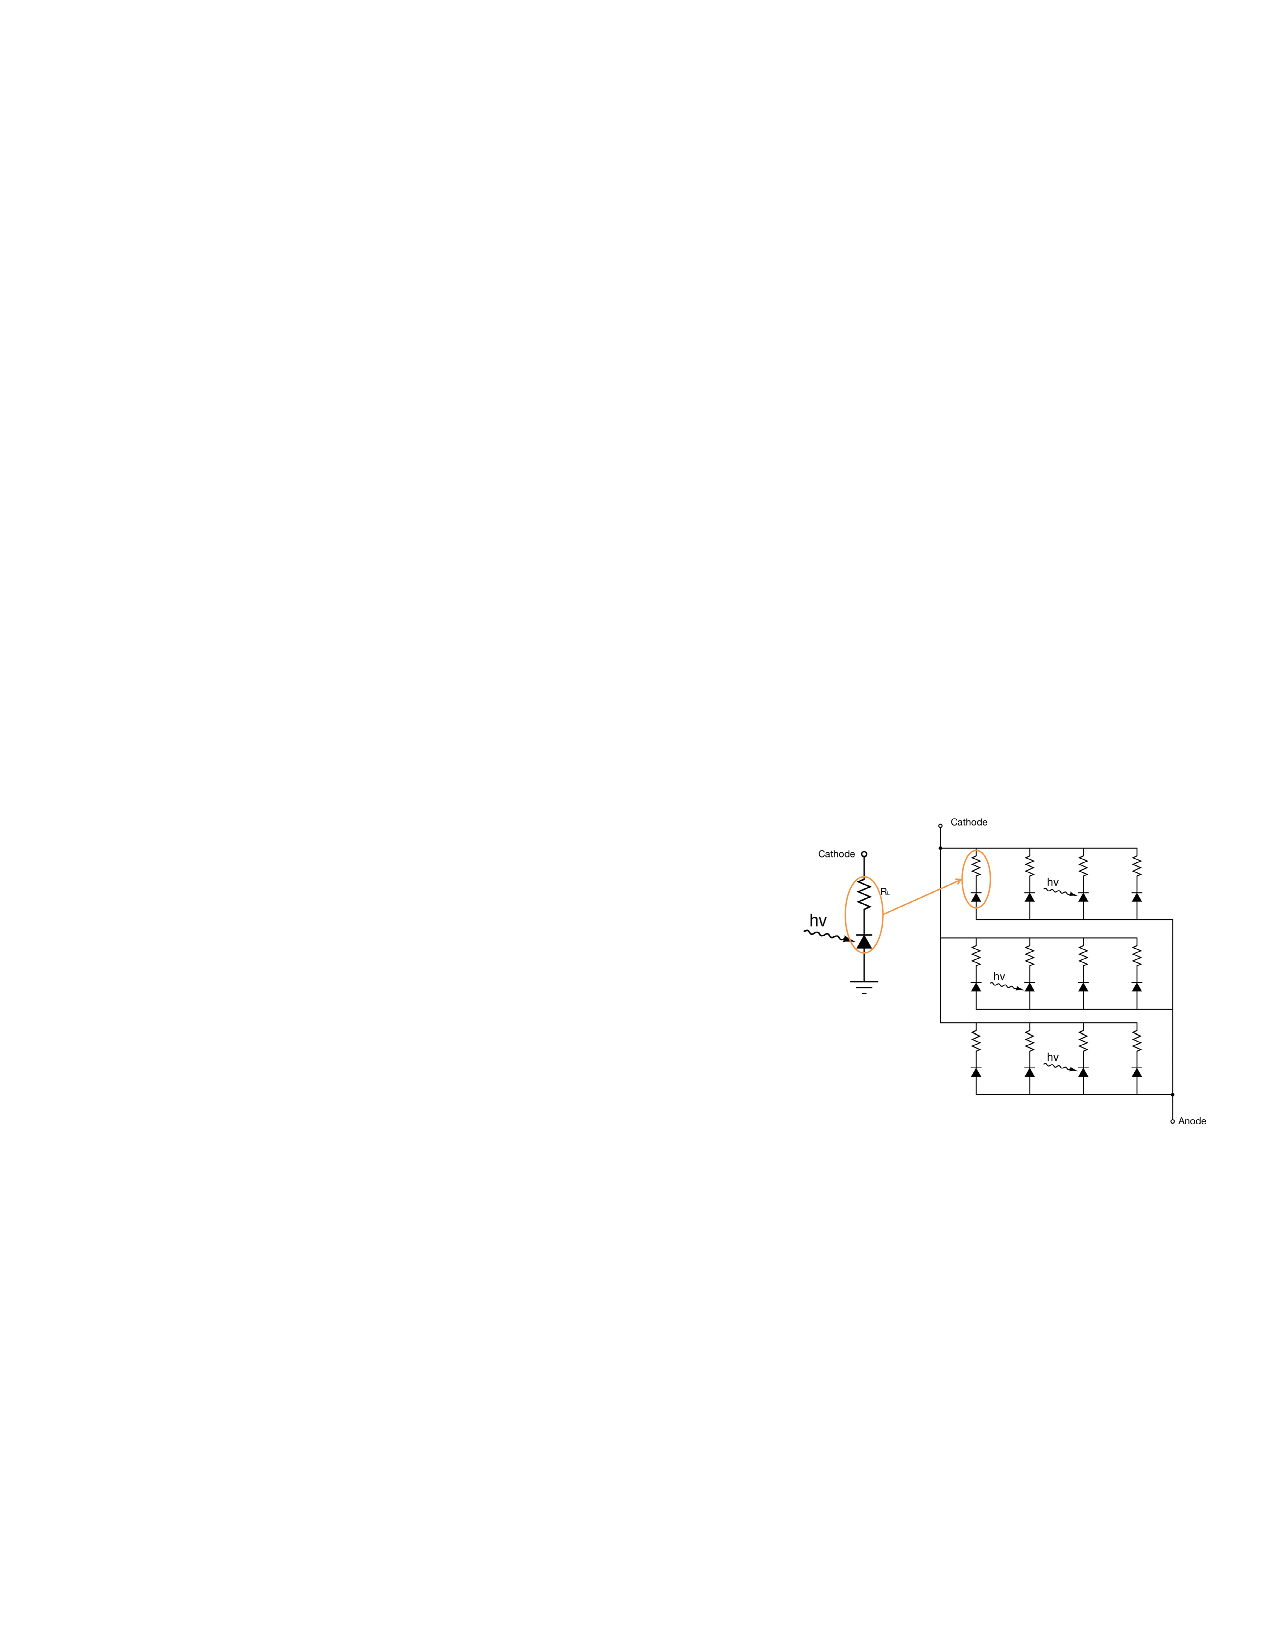
\includegraphics[scale=1.1]{img/SiPMCircuit.pdf}
	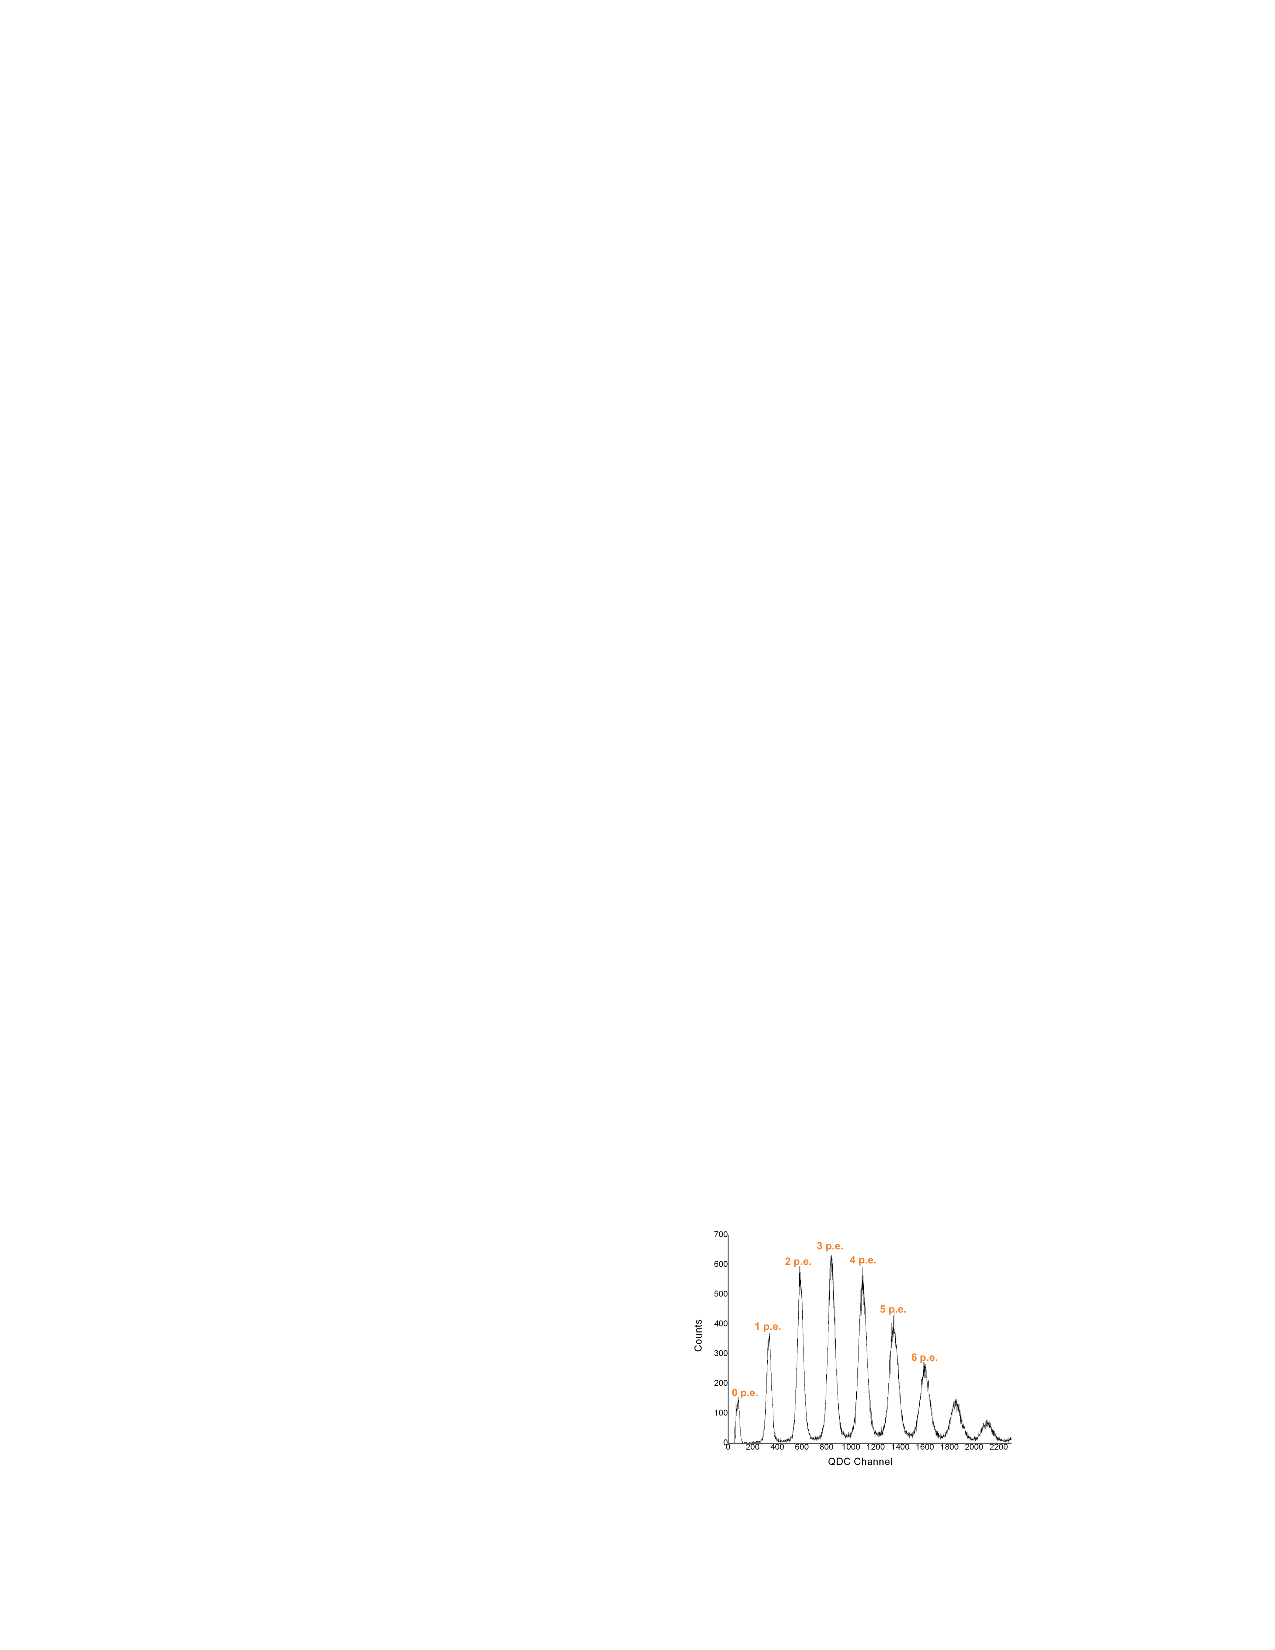
\includegraphics[scale=1.1]{img/PhotoelectronSpectrum.pdf}
	\caption{\label{fig.sipmc} Left: an array of microcells (photodiode plus quenching resistor) with their output summed up. Right: photoelectron spectrum of the SiPM, achieved using brief, low-level light pulses.}
\end{figure}

To overcome this lack of proportionality, the Silicon Photomultiplier integrates a dense array of small, electrically and optically isolated Geiger-mode photodiodes. Each photodiode element in the array is referred to as a ``microcell''. Depending on the application there can be between 100 and 1000 microcells per mm$^2$, each one with  its own quenching resistor. The signals of all microcells are then summed to form the output of the SPM. A simplified electric circuit to illustrate the concept is shown in Figure \ref{fig.sipmc} (left panel). Each microcell detects photons identically and independently. The sum of the discharge currents from each of these individual binary detectors combines to form a quasi-analog output, and is thus capable of giving information on the magnitude of an incident photon flux. The response to low-level light pulses is shown in in Figure \ref{fig.sipmc} (right panel).

\subsection{Silicon photomultipliers performance parameters}
The the main parameters that characterize a SiPM are: gain, PDE, noise, dynamic range, timing and temperature sensitivity. We briefly discuss those parameters here.

\subsubsection*{Over-Voltage}
The breakdown voltage (V$_{br}$) is the bias point at which the electric field strength generated in the depletion region is sufficient to create a Geiger discharge. The point of breakdown is clearly seen on an I-V plot by the sudden increase in current, as in 
Figure \ref{fig.sipp1} (left panel). The bias voltage (V$_{bias}$) is typically set at about 2V above the breakdown voltage. This 2V gap is referred to as the ``over-voltage'' 
($\Delta$V) and is critical in defining the important performance parameters of the SiPM.

\begin{figure}[!bhtp]
	\centering
	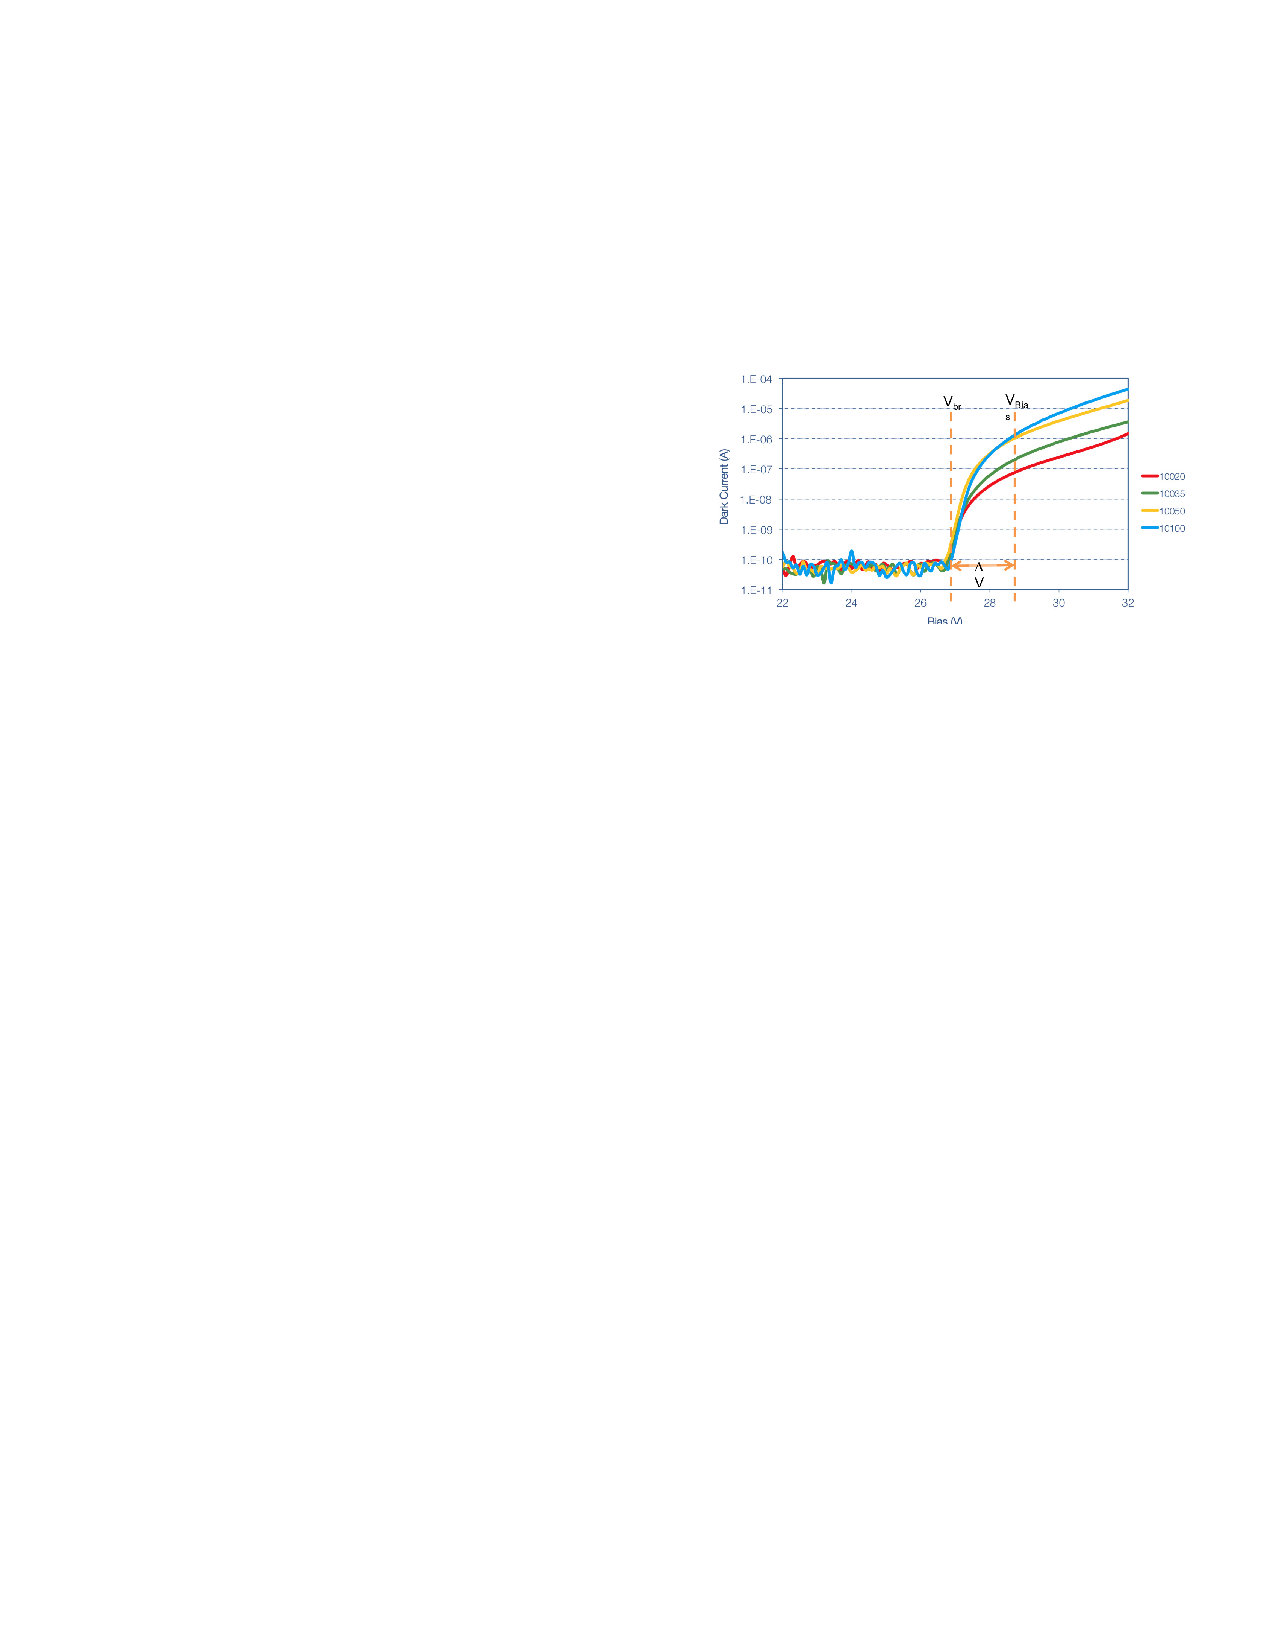
\includegraphics[scale=0.9]{img/SiPMVb.pdf}
	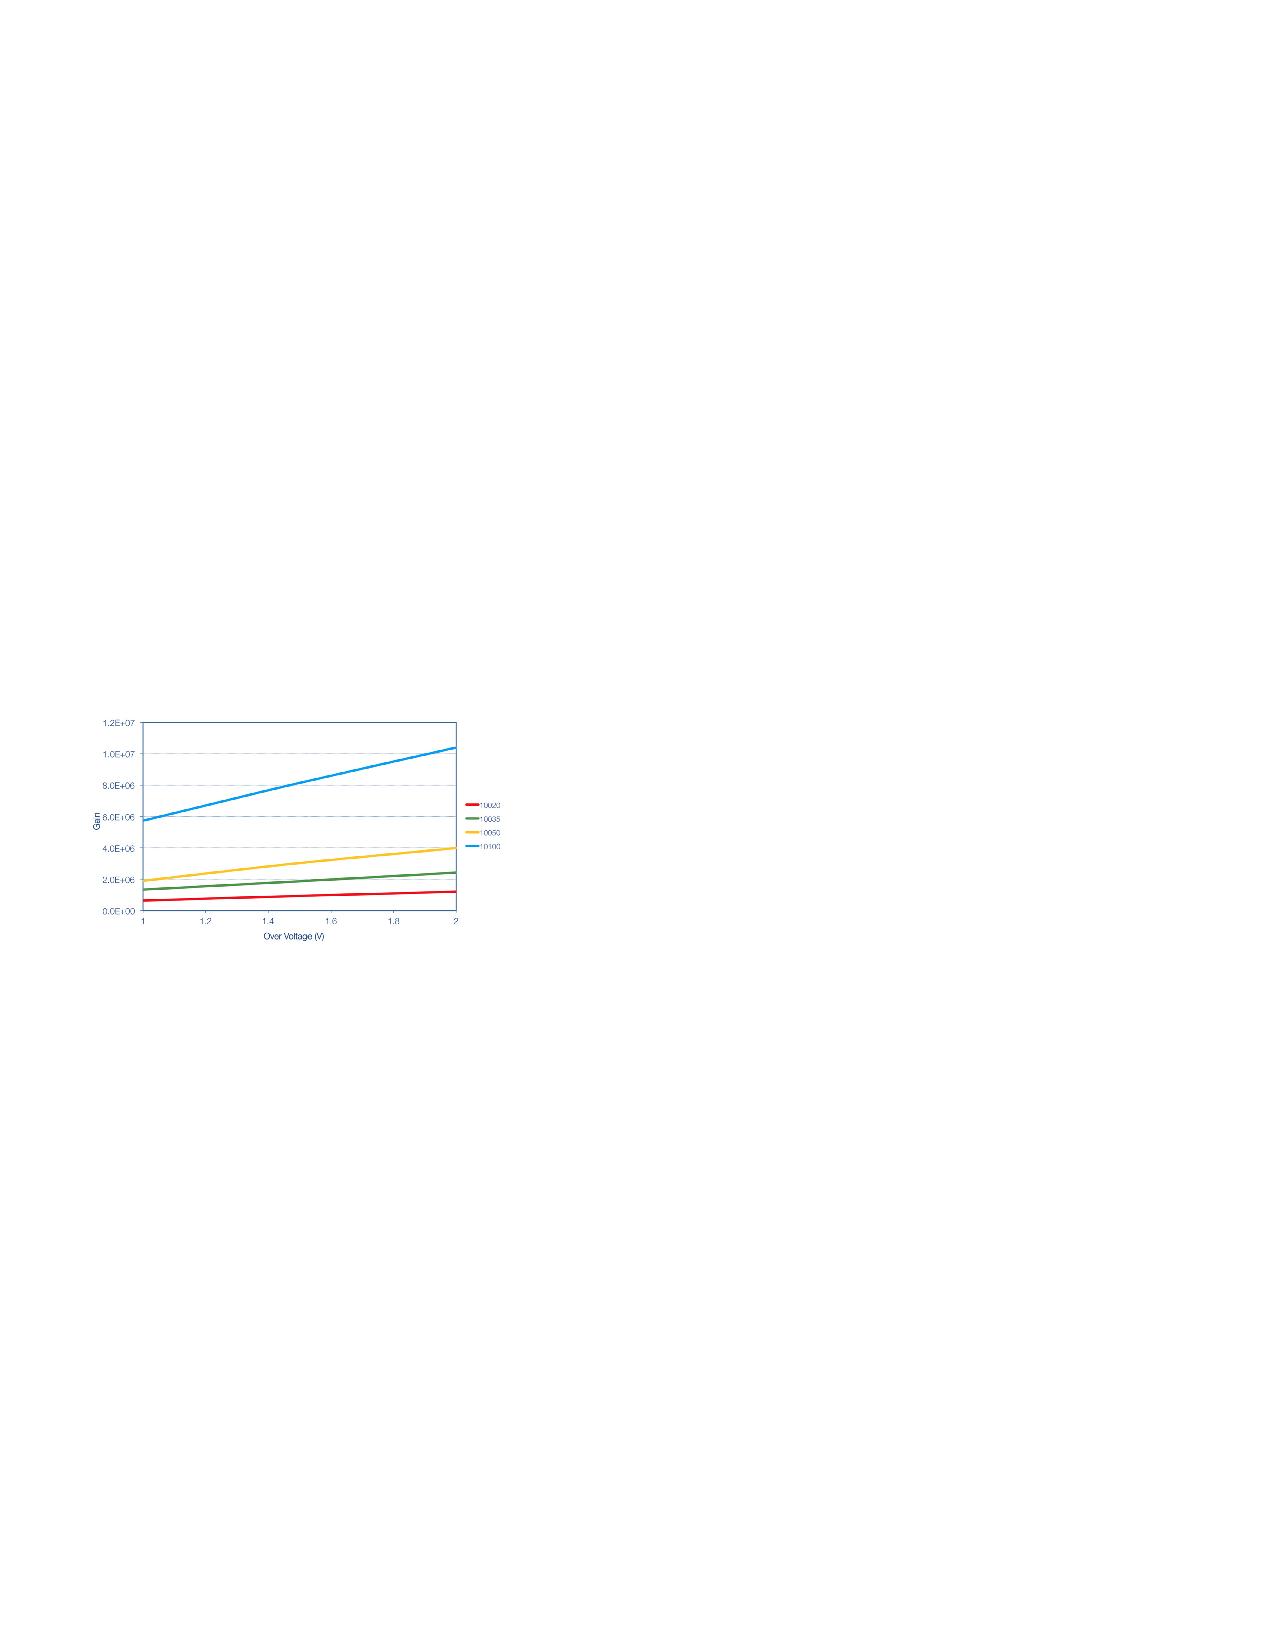
\includegraphics[scale=0.9]{img/SiPMGain.pdf}
	\caption{\label{fig.sipp1} Left: Dark current as a function of the voltage for 1 mm SiPMs of various microcell size (20 $\mu$m, 35 $\mu$m, 50 $\mu$m, 100 $\mu$m). Right: gain as a function of the over-voltage for various microcell size (20 $\mu$m, 35 $\mu$m, 50 $\mu$m, 100 $\mu$m).}
\end{figure}
\subsubsection*{Gain}

Each microcell in an SIPM is comprised of a Geiger-mode photodiode in series with an integrated quench resistor. Each microcell generates a highly uniform and quantized amount of charge every time the microcell undergoes a Geiger breakdown. The gain of a microcell (and hence the detector) is defined as the ratio of the output charge to the charge on an electron. The output charge can be calculated from the over-voltage and the microcell capacitance.

\begin{equation}
G = \frac{C \cdot \Delta V}{q}
\end{equation}

Figure \ref{fig.sipp1} (right panel) shows the gain as a function of the over-voltage  for
different microcell sizes. 

\subsubsection*{Photon Detection Efficiency (PDE)}

\begin{figure}[!bhtp]
	\centering
	
\includegraphics[scale=0.9]{img/SiPMPDE2.pdf}
	
	\caption{\label{fig.pde} PDE as a function of the wavelength for two different over-voltages.}
\end{figure}

The photon detection efficiency (PDE) of a SIPM is the statistical probability that an incident photon will produce a Geiger pulse from one of the SPM microcells. It differs slightly from the quantum efficiency (QE) that is quoted for a PMT or APD, due to the microcell structure of the device. The PDE is a function of wavelength and bias and is given by

\begin{equation}
PDE(\lambda, V) = \eta{\lambda} \cdot \epsilon(V) \cdot F
\end{equation}
%
where $ \eta{\lambda}$~is the quantum efficiency of silicon, $\epsilon(V)$~is the avalanche initiation probability and F is the fill factor of the device. The avalanche initiation probability takes into account the fact that no all generated photoelectrons will initiate an avalanche. The fill factor is the ratio of active to inactive area in the SiPM as a result of the gaps between microcells. The PDE of a typical SiPM is shown in Figure \ref{fig.pde} as a function of the wavelength for for two different over-voltages. The sensitivity of SiPMs peaks around 420 nm with a PDE nearing 45 \% for sufficiently high over-voltage. 

\subsubsection*{Noise}

\begin{figure}[!bhtp]
	\centering
	
\includegraphics[scale=0.9]{img/SiPMDCR.pdf}
	\caption{\label{fig.dcr} DCR as a function of the voltage for SENSL B series (blue line) and the new D series (red line) to be used in PETALO. Advances in SiPM manufacturing technology have reduced the DCR in more than one order of magnitude.}
\end{figure}


The main source of noise in an SPM is the dark count rate (DCR), which is primarily due to thermally generated electrons that create an avalanche in the high field region. The signals resulting from the breakdown of the cell, due to either photoelectrons or thermally generated electrons, are identical. Therefore, these electrons form a source of noise at the single photon level. If a threshold can be set above the single photon level, false triggers from the noise can be avoided, but the dark counts will always form a contribution to the measured signal.
Since this noise is comprised of a series of pulses, its magnitude
is often quoted as a pulse rate, typically in kHz or MHz. Figure \ref{fig.dcr} shows the DCR as a function of the voltage for SENSL B series (blue line) and the new D series (red line) to be used in PETALO. Advances in SiPM manufacturing technology have reduced the DCR in more than one order of magnitude. 

It should be noted that the magnitude of the DCR itself is not the noise contribution. If a given source of noise was always constant, then it could easily be subtracted from the signal. It is instead the fluctuations on the noise which degrade a measurement. The occurrence of the dark pulses is Poissonian in time and so the noise contribution can be taken as the square root of the DCR.

An additional component of SiPM noise is that of optical cross-talk between microcells. When undergoing avalanche, carriers near the junction emit photons as they are accelerated by the high electric field. These photons tend to be in the near infrared region and can travel substantial distances through the device. Typically $2 \times 10^5$ are emitted per electron crossing the junction. These photons can travel to neighboring microcells and may initiate a subsequent Geiger avalanche there. The crosstalk probability is the probability that an avalanching microcell will initiate an avalanche in a second microcell. The process happens instantaneously and as a consequence, single photons may generate signals equivalent to a 2, 3 or higher photoelectron event. The optical crosstalk probability is a function of SPM over-voltage and the distance between neighboring microcells, and can be estimated by the ratio of the count rate at the second photoelectron level to the count rate at the single photoelectron level. 

%\subsubsection*{Dynamic range and linearity}
%
%The dynamic range of a detector can be defined as the optical signal level range over which the detector provides a useful output. For a SiPM, this range extends from the lowest signal level detectable, to the optical signal level that results in all of the SiPM microcells detecting photons simultaneously (within the microcell dead-time). At this point the output signal completely saturates since no more microcells are available to detect incoming photons, until some of the microcells have recovered back to their sensitive (charged) state.
%
%The dynamic range of an SPM is therefore a function of the total number of microcells and the PDE of the device. Since the PDE of a SiPM is a function of the SiPM bias voltage and wavelength of the incident photons, the dynamic range of an SiPM is also a function of these parameters. The number of microcells fired as a function of the number of incident photons can be approximated by the expression:
%
%
%\begin{equation}
%M_{fired}(M,V,\lambda) = M \left( 1 - \exp\left({-\frac{PDE(V,\lambda) \cdot N_{ph}}{M}}\right)\right)
%\end{equation}
%%
%where N$_{fired}$~ is the number of microcell fired, N$_{ph}$~ is the number of incident photons, M is the number of SIPM microcells and PDE is the SPM photon detection efficiency. The expression also assumes that the incoming photons are evenly distributed across the surface of the SiPM. Above a certain signal level, and before saturation, the SPM response becomes sub-linear. This is because the output pulse of a single microcell is independent of the number of incident photons that initiated the output pulse. As the number of incident photons per microcell per second increases, the probability increases that two or more photons will interact in the same microcell at the same time. The SPM output begins to saturate when the number of detected photons begins to approach the number of microcells (M).
%
%\subsubsection*{Pulse shape}
%
%
%\begin{figure}[!bhtp]
%	\centering
%	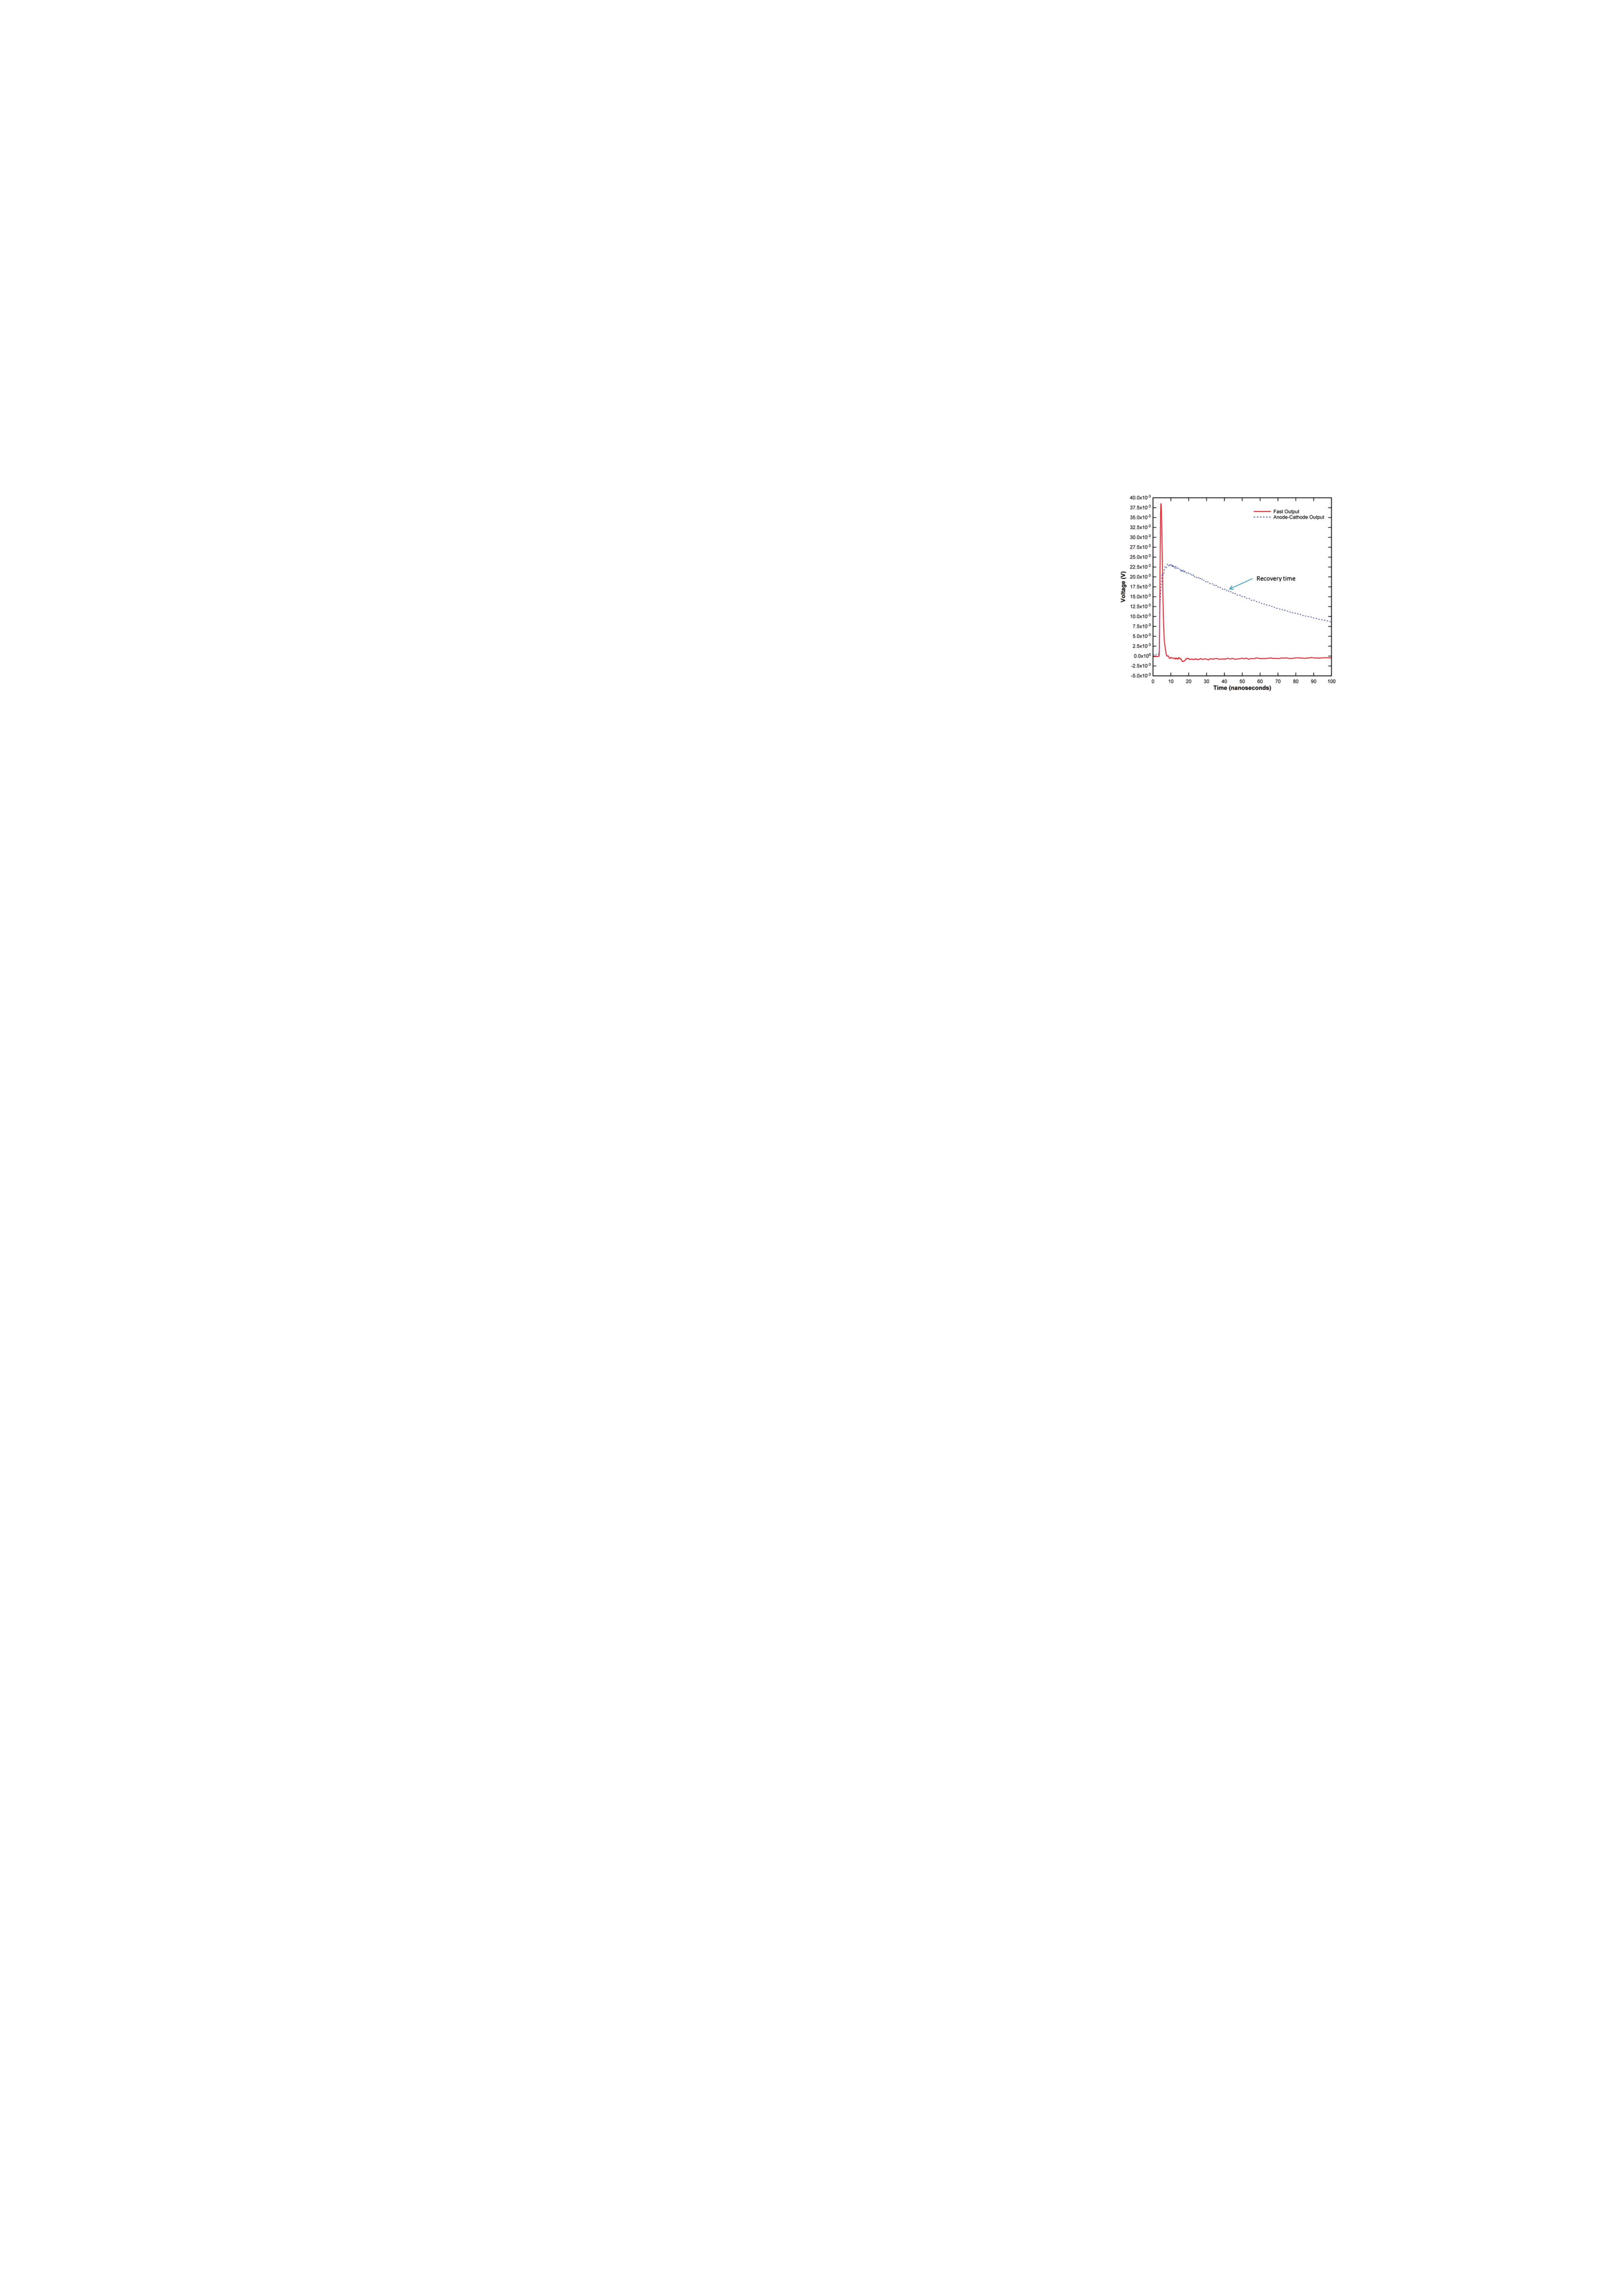
\includegraphics[scale=0.8]{img/TimeResponseSiPM.pdf}
%	
%	\caption{\label{fig.fr} Time response of a SENSL SiPM. The blue line represents the standard output, with a rise time of the order of 10 ns. The red line is the fast output available in this devices, with a rise time of 1 ns.}
%\end{figure}
%
%The rise time of a  SiPM depends upon the total area of device, and specifically, the capacitance resulting from the tracks that connect all of the microcells. The rise time varies from $\sim$~ 1 ns for to $\sim$ 10ns, depending on the area of the SiPM and of the technique used (Figure \ref{fig.fr}).
%
\subsubsection*{Temperature dependence}

The most important effect of temperature on the SiPM are a change in the breakdown voltage of the diode and in the dark count rate.

\begin{figure}[!bhtp]
	\centering
	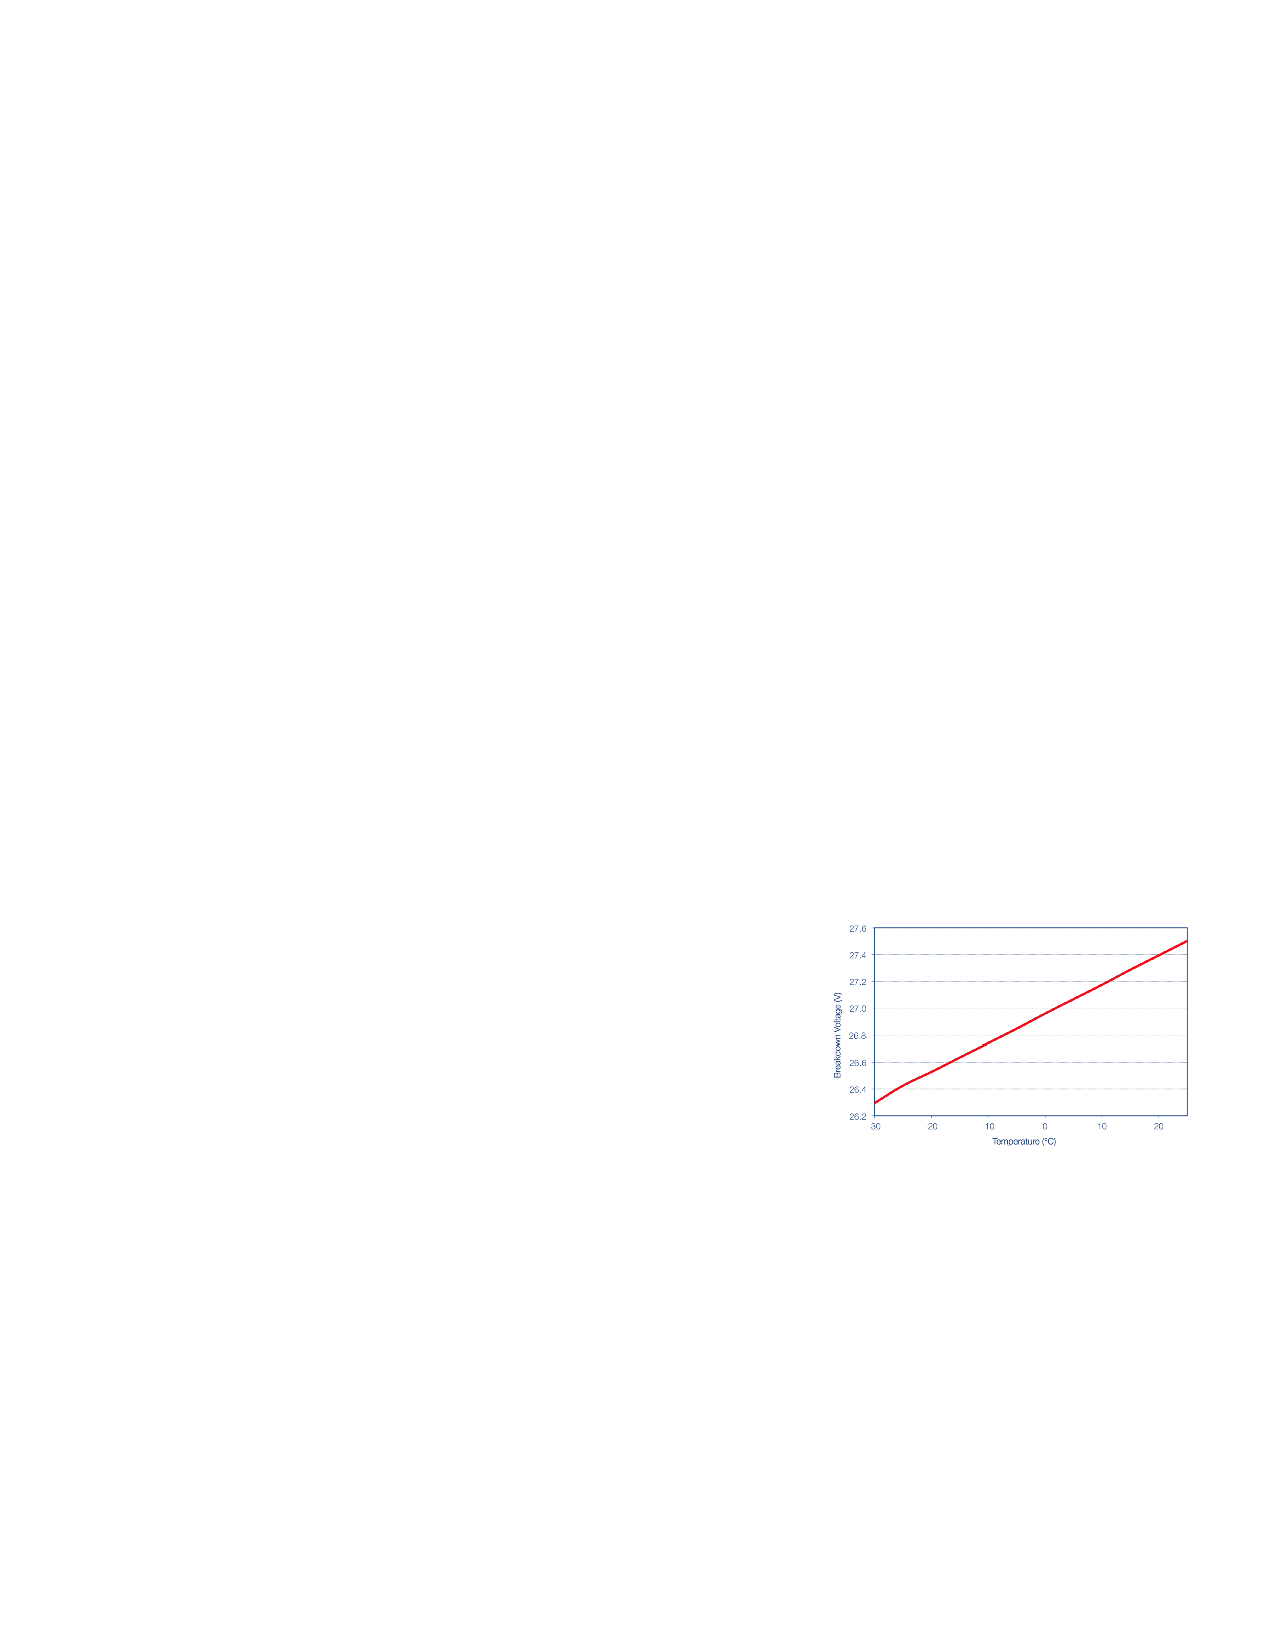
\includegraphics[scale=0.9]{img/VbTdep.pdf}
	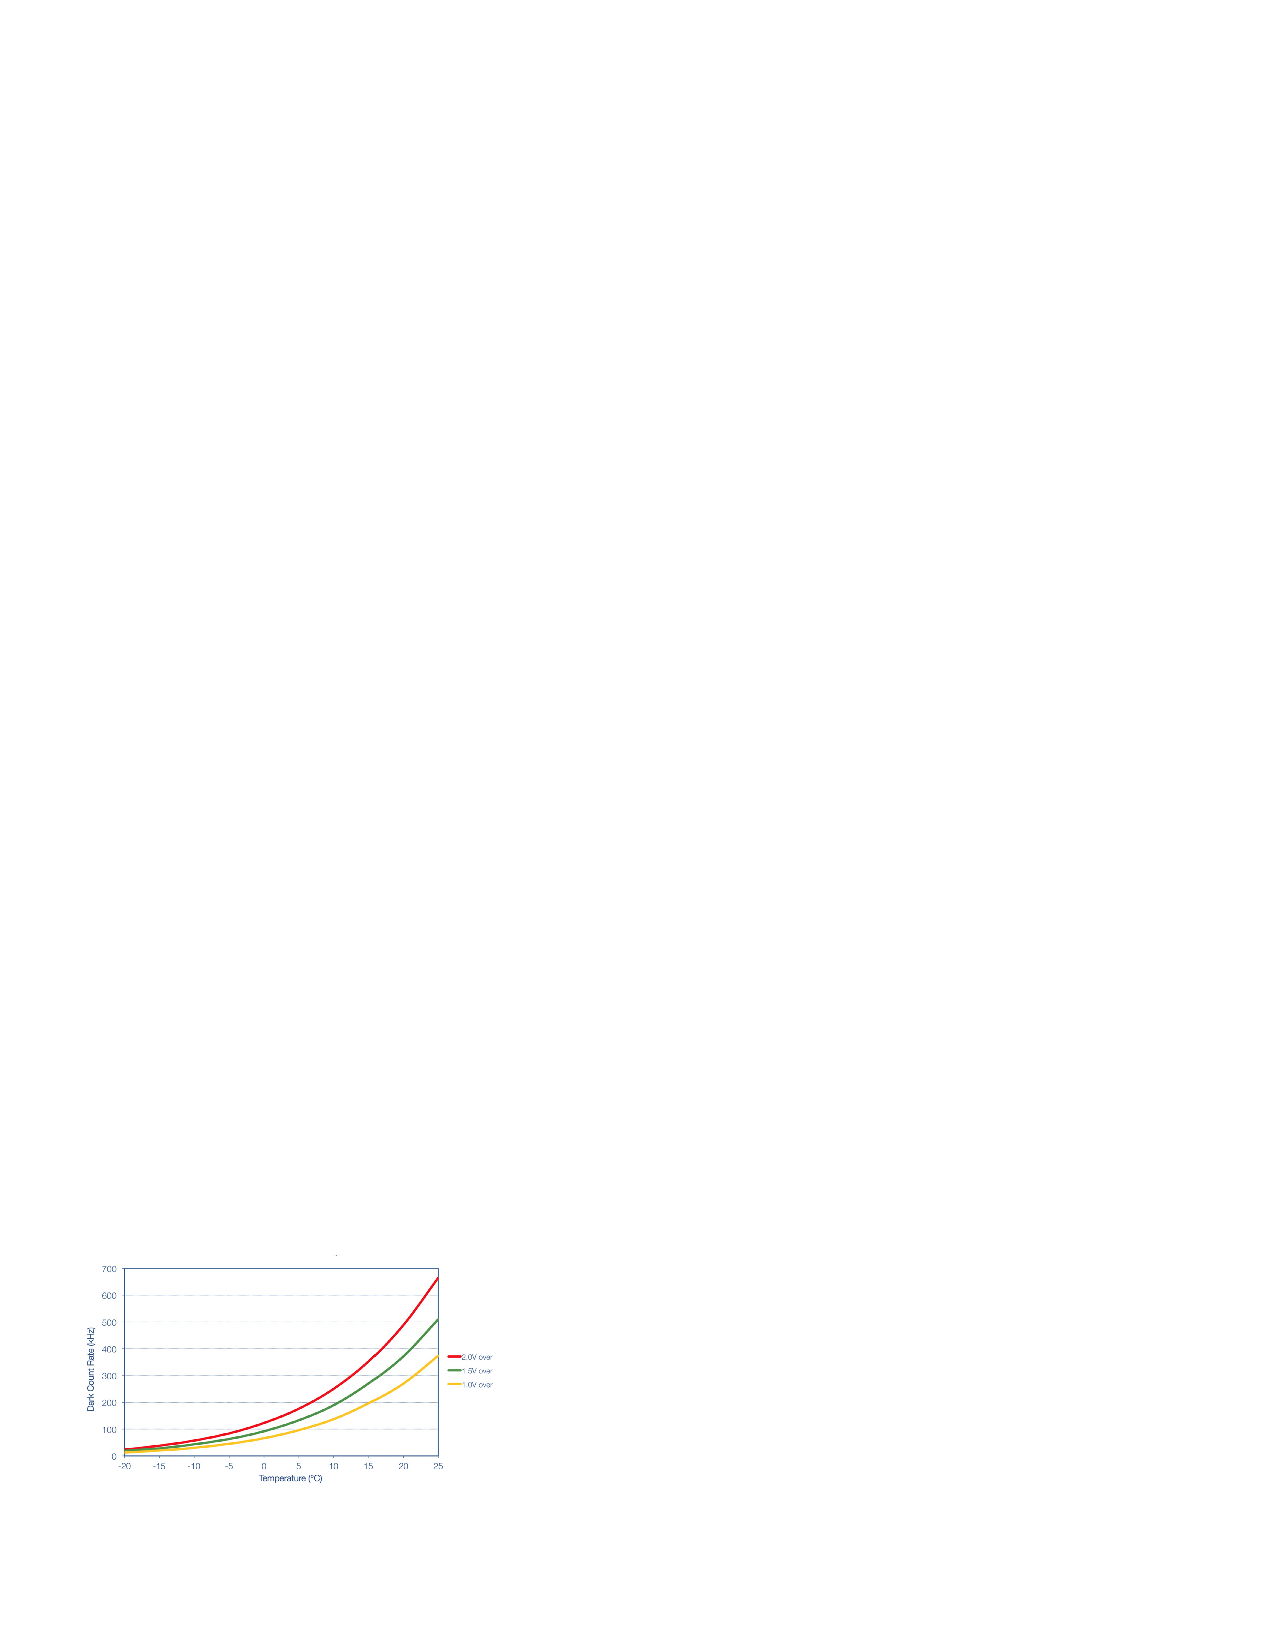
\includegraphics[scale=0.9]{img/DCRTdep.pdf}
	\caption{\label{fig.temp} Left: breakdown voltage as a function of the temperature. Right: DCR as a function of the temperature and over-voltage.}
\end{figure}


The breakdown voltage changes as a function of temperature, as shown in Figure \ref{fig.temp} (left panel). If a constant over-voltage is maintained, many parameters, such as gain, PDE and timing, will remain the same as at room temperature. However, regardless of constant over-voltage, the DCR will be altered by a change in temperature, as shown in Figure \ref{fig.temp} (right panel). An increase in temperature will increase dark rate, and the converse is also true: for every 10$^\circ$ C reduction in device temperature, the dark count rate by a factor 2. 

